\documentclass[12pt,a4paper]{report}
\usepackage[Rejne]{fncychap}
\usepackage{titlesec}
\usepackage{biblatex}
\usepackage[utf8]{inputenc}
\usepackage[french]{babel}
\usepackage[T1]{fontenc}
\usepackage{amsmath}
\usepackage{amsfonts}
\usepackage{amssymb}
\usepackage{graphicx}
\usepackage{fullpage}
\usepackage{caption}
\usepackage{subcaption}
\usepackage[left=2cm,right=2cm,top=2cm,bottom=2cm]{geometry}
\usepackage{ragged2e}
\author{BERJOLA Matthias 37000961-ADOLPHE Benjamin 37001213}           %   



\begin{document}
\title{Projet Développement mobile: Planee}
\author{BERJOLA MATTHIAS 37000961 - ADOLPHE BENJAMIN 37001213}
\date{\today} 

\maketitle


\newpage

\tableofcontents

\chapter{Introduction}  
\begin{flushleft}
\justify
Cette année, afin de valider l'UE développement mobile 2, nous avons dû réaliser un projet. Ce projet consistait à réaliser une application ou un jeu respectant certaines contraintes:
\begin{itemize}
\item[•] Le choix de l'application est laissé libre, mais une partie de la notation portera sur sa complexité (quelque chose de trop simpliste ne donnera pas lieu à beaucoup de points).
\item[•] L’application doit proposer : plusieurs écrans, une présentation
sous forme de liste, une sauvegarde persistante.
\item[•] L’application doit fonctionner correctement sur tout type d’écran (grand, petit…), en mode portrait et paysage : ressources alternatives sous Android + contraintes sur les composants graphiques.
\end{itemize}
De ce fait mon collègue et moi même avons opté pour une application. Après un BrainStorming intensif, nous avons décidé d'appeler notre application Planee et nous expliquerons son fonctionnement par la suite.
\end{flushleft}

\newpage
\chapter{L'application Planee}
\section{Principe}
\begin{flushleft}
\justify
Planee est une application de gestion d'évènements. Elle permettra à l'utilisateur d'organiser et créer ses différents évènements. En effet, chaque évènement est composé d'un titre, d'une date limite de tâches et chaque tâche est composée d'un titre, d'un nom de magasin et éventuellement d'une URL indiquant le site du magasin si l'utilisateur a besoin de passer une commande. Sur le long terme l'application devrait supposer des magasins ou différents sites pour passer commande.
\end{flushleft}
\section{Architecture de l'application}
\begin{flushleft}
\justify
L'application Planee est structurée en 3 Activités:
\begin{itemize}
\item[•] L'activité MainActivity représente la page d'Accueil.
\item[•] L'activité AddActivity représente la page d'ajout d'un évènement.
\item[•] L'activité DetailActivity représente la page de détails d'un évènement.
\end{itemize}
\end{flushleft}
\subsection{MainActivity}
\begin{flushleft}
\justify
Comme dit précédemment la MainActivity représente la page d'accueil. En effet, la MainActivity est composée principalement d'un élément ListView. La ListView permettra de lister les différents évènements. Les évènements sont récupérés dans la Base de Données locale du téléphone, si aucun évènement est présent dans la Base de Donnée alors un message apparaîtra à l'écran.\\

Quelques fonctionnalités de la page d'accueil:
\begin{itemize}
\item[•] Appuie long sur un évènement pour le supprimer
\item[•] Appuie sur un évènement pour avoir les détails suivants:
\begin{itemize}
\item[•] Nom de l'évènement
\item[•] Date de l'évènement
\item[•] Liste des taches de l'évènement
\end{itemize}
\item[•] Appuie sur le bouton retour pour quitter l'application
\end{itemize}
\begin{figure}[!h]
    \centering
    \begin{subfigure}[b]{0.3\textwidth}
        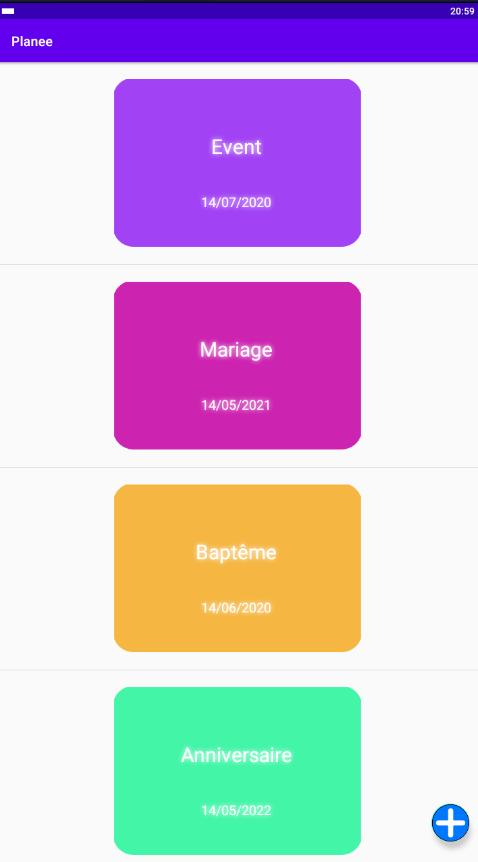
\includegraphics[width=\textwidth]{HomeWEvents}
    \end{subfigure}
    \begin{subfigure}[b]{0.3\textwidth}
        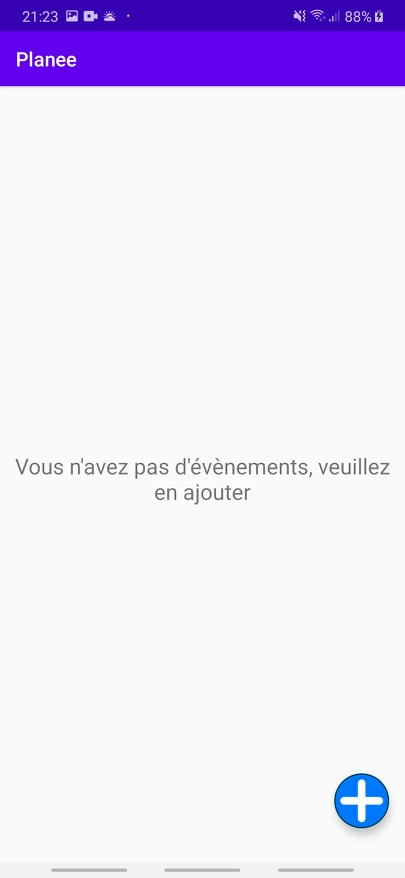
\includegraphics[width=\textwidth]{HomeNoEvent}
    \end{subfigure}
    \caption{Page d'accueil avec et sans évènements}
\end{figure}
\end{flushleft}
\subsection{AddActivity}
\begin{flushleft}
\justify
La page contient un formulaire permettant d'entrer le nom, la date limite de l'évènement, l'heure et l'ensemble des tâches. Le formulaire d'ajout de tâches est dynamique grâce au bouton "Nouvelle tâche".\\

Quelques fonctionnalités du formulaire:
\begin{itemize}
\item[•] Appuie sur le bouton "Nouvelle tâche" afin d'ajouter un champs de saisie d'une nouvelle tâches, ces champs sont composées de 3 champs de saisie de textes:
\begin{itemize}
\item[•] Nom de la tâche
\item[•] Potentiellement le nom du magasin
\item[•] Potentiellement l'URL du site du magasin
\end{itemize}
\item[•] Appuie sur le bouton "Ajout de l'évènement" afin d'ajouter l'évènement dans la base de données locale de l'appareil et déclencher une alarme à la date et l'heure entrées par l'utilisateur (Voir partie problèmes rencontrés)
\end{itemize}
\begin{figure}
    \centering
    \begin{subfigure}[b]{0.3\textwidth}
        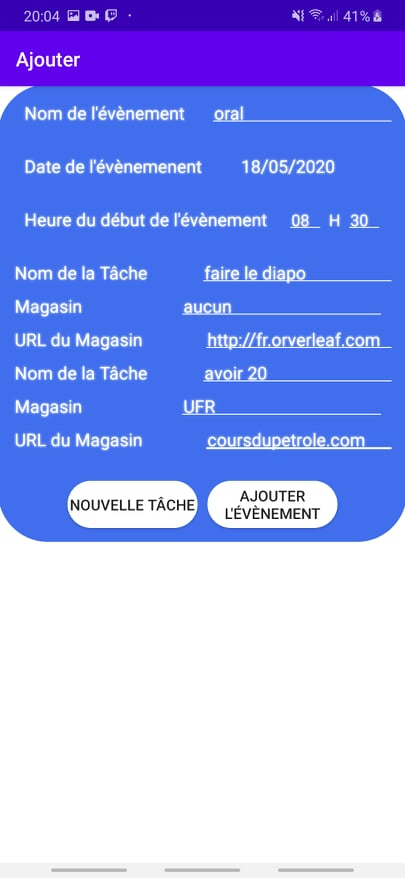
\includegraphics[width=\textwidth]{FormWTask}
    \end{subfigure}
    \begin{subfigure}[b]{0.3\textwidth}
        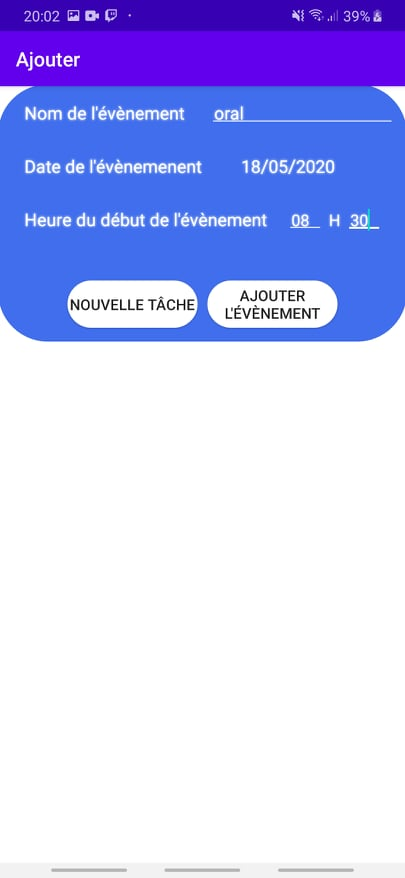
\includegraphics[width=\textwidth]{FormNoTask}
    \end{subfigure}
    \caption{Page du formulaire d'ajout avec et sans tâches}
\end{figure}
\end{flushleft}
\newpage
\subsection{DetailsActivty}
\begin{flushleft}
\justify
Comme dit dans la partie concernant la MainActivity, lors d'un appui sur un évènement on accède à la page de détails de cet évènement. Ainsi, on va récupérer tout les éléments dans la Base de données locale en rapport avec cet évènement.
\end{flushleft}
\subsection{Bases de données}
\begin{flushleft}
\justify
Pour ce projet, nous avons utilisé une base de données composée de 2 tables:
\begin{itemize}
\item[•] Une table Event\_Table
\item[•] Une table Tache\_Table
\end{itemize}
\medskip
La table Event\_Table sert à stocker les différents évènements créé. À l'intérieur on y trouve :
\begin{itemize}
\item[•] l'id de l'évènement
\item[•] Le nom de l'évènement
\item[•] Sa date limite(La date où l'évènement se produira)
\item[•] L'heure limite (L'heure à laquelle l'évènement se déroulera)
\end{itemize}
\medskip 
La table Tache\_Table sert quand à elle à stocker les différentes tâches à stocker les différentes tâches à effectuer afin de préparer l'évènement convenablement. Elle est composée de:
\begin{itemize}
\item[•] L' id de la tâche
\item[•] Du nom du magasin dans lequel la tâche doit être effectué
\item[•] De l'URL du magasin si l'achat peut être effectuer en ligne
\item[•] IdEvent qui est une clé étrangère permettant de savoir à quel évènement appartient la tâche
\end{itemize}
\medskip 
On trouve également deux méthodes indispensables à la base de données :
\begin{itemize}
\item[•] La méthode InsertEvent
\item[•] La méthode getAllEvent
\end{itemize}
\medskip 
La première méthode a été crée dans le but de pouvoir insérer chaque événements(composé de tâches) dans la base de données. La seconde méthode permet de récupérer tout les évènements crées par l'utilisateur afin de pouvoir les afficher de nouveau lorsque l'utilisateur reviens sur l'application après l'avoir fermé. \\
Le choix d'une base données a été fait dans le but de garantir la persistance des données de l'utilisateur à chaque fois que l'application est quittée puis ré-ouverte.

\begin{figure}[!h]
    \centering
    \begin{subfigure}[b]{0.3\textwidth}
        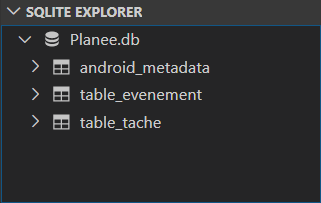
\includegraphics[width=\textwidth]{SchemaBDD}
    \end{subfigure}
    \begin{subfigure}[b]{0.3\textwidth}
        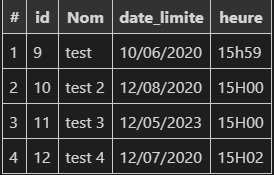
\includegraphics[width=\textwidth]{TableEvent}
    \end{subfigure}
    \begin{subfigure}[b]{0.3\textwidth}
        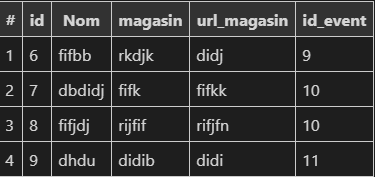
\includegraphics[width=\textwidth]{TableTache}
    \end{subfigure}
    \caption{Schéma de la Base de données}
\end{figure}
\end{flushleft}
\section{Problèmes rencontrés}
\begin{flushleft}
\justify
Au cours de ce projet, nous avons rencontré plusieurs problèmes. Nous allons donc citer dans ce rapports les différents problèmes que nous avons rencontré.
\end{flushleft}
\subsection{Fragments}
\begin{flushleft}
\justify
Au début de ce projet, lors du choix de la première activité, nous avons choisi l'activité "Navigation Drawer Activity".\\
\center
\begin{minipage}{0.48\linewidth}
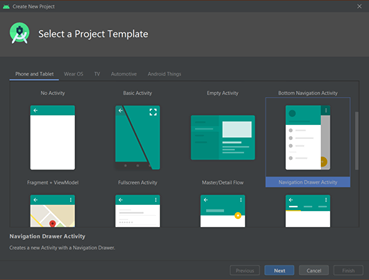
\includegraphics[width=\linewidth]{Template}
\captionof{figure}{Template}
\end{minipage}
\justify
Cependant, ce template est basé sur l'utilisation des 
Fragments qui est une notion pas vue en cours.
\end{flushleft}
\subsection{Notifications}
\subsection{Layout}
\begin{flushleft}
\justify
Lors de la réalisation du design de l'application nous devions géré en plus des éléments de bases(couleurs formes etc) les layouts. Deux problèmes revenais souvent: La conservation de l'échelle lorsque l'on passe à un appareil plus petit et la superposition des éléments lors de ce passage.\\
Au départ le design de l'application était réalisé entièrement avec des ConstraintLayout. Le problème avec les Constraint Layout est le manque de précision et de rigidité dans les contraintes que nous mettons. De ce fait des éléments qui semblait bien placés se retrouvait déplacés sans aucune intervention de notre part lorsque nous lançons l'application. Nous avons donc pris la décision de remplacer les Constraint Layout par des Relative Layout là où cela posait problème(page détail, page addDétail notamment). Après ce changement nous avons pu convenablement placé les différents éléments sans erreurs apparentes.
\end{flushleft}
\section{Amélioration futures}
\newpage
\chapter{Conclusion}
\newpage
\chapter{Bibliographie}
\end{document}
